\documentclass[letterpaper]{article}
\usepackage[top=1.0in,bottom=1.0in,left=1.0in,right=1.0in]{geometry}
\usepackage{verbatim}
\usepackage{amssymb}
\usepackage{graphicx}
\usepackage{longtable}
\usepackage{amsfonts}
\usepackage{amsmath}
\usepackage{hyperref}
\usepackage{subfigure}
\usepackage{booktabs}
\def\thesection       {\arabic{section}}
\def\thesubsection     {\thesection.\alph{subsection}}

\author{Roberto E. Fairhurst Agosta
        \\ \href{mailto:ref3@illinois.edu}{\texttt{ref3@illinois.edu}}
}

\title{NPRE 555\\ Computer Project 2}
\begin{document}
%\clearpage
\begin{titlepage}
\maketitle
\thispagestyle{empty}
\end{titlepage}

\section{Introduction}

This computer project calculated the neutron flux in a moderator slab using the P$_N$ approximation.
Table \ref{tab:parameters} summarizes the input parameters.
The following sections define the equations for each P$_N$ approximation.

\begin{table}[htbp!]
  \centering
  \caption{Input parameters.}
  \begin{tabular}{lcc}
  \toprule
                 & Value & Units   \\
  \midrule
  Slab thickness (L) & 8     & cm  \\
  $\Sigma_t$     & 1.0   & 1/cm    \\
  $\Sigma_{s0}$  & 0.4   & 1/cm    \\
  $\Sigma_{s1}$  & 0.1   & 1/cm    \\
  $\Sigma_{s2}$  & 0.1   & 1/cm    \\
  $\Sigma_{s3}$  & 0.1   & 1/cm    \\
  q$_0$          & 1     & n/cm$^{3}$/s \\
  \bottomrule
  \end{tabular}
  \label{tab:parameters}
\end{table}

\section{P$_1$ approximation}

\begin{align}
    & \frac{d}{dx}\phi_1 + \Sigma_0 \phi_0 = q_0  \label{eq:P1-0} \\
    & \frac{d}{dx}\phi_0 + 3 \Sigma_1 \phi_1 = 0  \label{eq:P1-1} \\
    \intertext{where}
    & \Sigma_n = \Sigma_t - \Sigma_{sn} \notag
\end{align}

\subsection{P$_1$ approximation Marshak boundary condition}
\label{sec:p1-marshak}

\begin{align}
    & \frac{1}{4}\phi_0 (x=0) + \frac{1}{2}\phi_1 (x=0)  = 0   \\
    & -\frac{1}{4}\phi_0 (x=L) + \frac{1}{2}\phi_1 (x=L) = 0
\end{align}

\subsection{P$_1$ approximation Mark boundary condition}
\label{sec:p1-mark}

\begin{align}
    & \frac{1}{2}\phi_0 (x=0) + \frac{3}{2}\phi_1 (x=0) \mu_0 = 0  \\
    & \frac{1}{2}\phi_0 (x=L) + \frac{3}{2}\phi_1 (x=L) \mu_1 = 0  \\
    \intertext{where}
    & \mu_{0,1} = \pm 0.57735 \notag
\end{align}

\subsection{Numerical method}

Through some algebraic manipulation of Equations \ref{eq:P1-0} and \ref{eq:P1-1}, the method obtains the following equation.
The solver discretizes the equation with the finite difference method.
Equation \ref{eq:P1-1} combined with the boundary condition equations (Sections \ref{sec:p1-marshak} and \ref{sec:p1-mark}) allow to impose the boundary conditions on the numerical solution.

\begin{align}
    & -\frac{d}{dx}\left(\frac{1}{3\Sigma_1} \frac{d}{dx}\phi_0 \right) + \Sigma_0 \phi_0 = q_0
\end{align}

\section{P$_3$ approximation}

\begin{align}
    & \frac{d}{dx}\phi_1 + \Sigma_0 \phi_0 = q_0  \label{eq:P3-0} \\
    & 2 \frac{d}{dx}\phi_2 + \frac{d}{dx}\phi_0 + 3 \Sigma_1 \phi_1 = 0  \label{eq:P3-1} \\
    & 3 \frac{d}{dx}\phi_2 + 2\frac{d}{dx}\phi_1 + 5 \Sigma_2 \phi_2 = 0 \label{eq:P3-2} \\
    & 3\frac{d}{dx}\phi_2 + 7 \Sigma_3 \phi_3 = 0  \label{eq:P3-3} \\
    \intertext{where}
    & \Sigma_n = \Sigma_t - \Sigma_{sn} \notag
\end{align}

\subsection{P$_3$ approximation Marshak boundary condition}
\label{sec:p3-marshak}

\begin{align}
    & \frac{1}{2}\phi_0 (x=0) + \phi_1 (x=0) + \frac{5}{8}\phi_2 (x=0) = 0   \\
    & -\frac{1}{8}\phi_0 (x=0) + \frac{5}{8}\phi_2 (x=0) + \phi_3 (x=0) = 0  \\
    & -\frac{1}{2}\phi_0 (x=L) + \phi_1 (x=L) - \frac{5}{8}\phi_2 (x=L) = 0  \\
    & \frac{1}{8}\phi_0 (x=L) - \frac{5}{8}\phi_2 (x=L) + \phi_3 (x=L) = 0
\end{align}

\subsection{P$_3$ approximation Mark boundary condition}
\label{sec:p3-mark}

\begin{align}
    & \frac{1}{2}\phi_0 (x=0) P_0(\mu_0) + \frac{3}{2}\phi_1 (x=0) P_1(\mu_0) + \frac{5}{2}\phi_2 (x=0) P_2(\mu_0) + \frac{7}{2}\phi_3 (x=0) P_3(\mu_0) = 0  \\
    & \frac{1}{2}\phi_0 (x=0) P_0(\mu_1) + \frac{3}{2}\phi_1 (x=0) P_1(\mu_1) + \frac{5}{2}\phi_2 (x=0) P_2(\mu_1) + \frac{7}{2}\phi_3 (x=0) P_3(\mu_1) = 0  \\
    & \frac{1}{2}\phi_0 (x=L) P_0(\mu_2) + \frac{3}{2}\phi_1 (x=L) P_1(\mu_2) + \frac{5}{2}\phi_2 (x=L) P_2(\mu_2) + \frac{7}{2}\phi_3 (x=L) P_3(\mu_2) = 0  \\
    & \frac{1}{2}\phi_0 (x=L) P_0(\mu_3) + \frac{3}{2}\phi_1 (x=L) P_1(\mu_3) + \frac{5}{2}\phi_2 (x=L) P_2(\mu_3) + \frac{7}{2}\phi_3 (x=L) P_3(\mu_3) = 0  \\
    \intertext{where}
    & P_0(\mu) = 1    \notag \\
    & P_1(\mu) = \mu  \notag \\
    & P_2(\mu) = \frac{1}{2} (3\mu^2-1)    \notag \\
    & P_3(\mu) = \frac{1}{2} (5\mu^3-\mu)  \notag \\
    & \mu_{0,1,2,3} = [ 0.86114, 0.33998, -0.33998, -0.86114 ] \notag
\end{align}

\subsection{Numerical method}

Through some algebraic manipulation of Equations \ref{eq:P3-0} to \ref{eq:P3-3}, the method obtains the following equations.
The solver discretizes the equations with the finite difference method.
To solution of the coupled system used an explicit solver based on the previous iteration solution, requiring an iterative solver.
The convergence criteria was an $L_2$-norm of the relative difference between fluxes smaller than $1 \times 10^{-6}$.
Equations \ref{eq:P3-1} and \ref{eq:P3-3} combined with the boundary condition equations (Sections \ref{sec:p3-marshak} and \ref{sec:p3-mark}) allow to impose the boundary conditions on the numerical solution.

\begin{align}
    & -\frac{d}{dx}\left(\frac{1}{3\Sigma_1} \frac{d}{dx}\phi_0 + \frac{2}{3\Sigma_1} \frac{d}{dx}\phi_2 \right) + \Sigma_0 \phi_0 = q_0   \\
    & -\frac{d}{dx}\left(\frac{2}{3\Sigma_1} \frac{d}{dx}\phi_0 + \left(\frac{4}{3\Sigma_1} + \frac{9}{7\Sigma_3} \right) \frac{d}{dx}\phi_2 \right) + 5 \Sigma_2 \phi_2 = 0
\end{align}

\section{Results}

Figure \ref{fig:results} displays the scalar flux for all the approximations with the different boundary conditions.
Figure \ref{fig:a} shows a full range plot of all the approximations normalized to their maximum value.
Figure \ref{fig:b} exhibits a reduced range plot close to the right boundary for a better appreciation of the boundary condition effects.
P$_3$ flux has a larger magnitude than P$_1$ flux away from the boundaries, which indicates that lower P$_N$ approximation fluxes have rounder shapes.
A rounder shape is an indicator of poorer neutron conservation.
Additionally, imposing a Mark boundary condition causes the scalar flux to have a smaller magnitude than the Marshak boundary condition case.
A smaller flux on the boundary is a sign of `more neutrons' leaving the domain, which indicates that the Marshak boundary condition better preserves the neutrons in the domain.

\begin{figure}[h!]
        \centering
        \subfigure[Full range plot. \label{fig:a}]{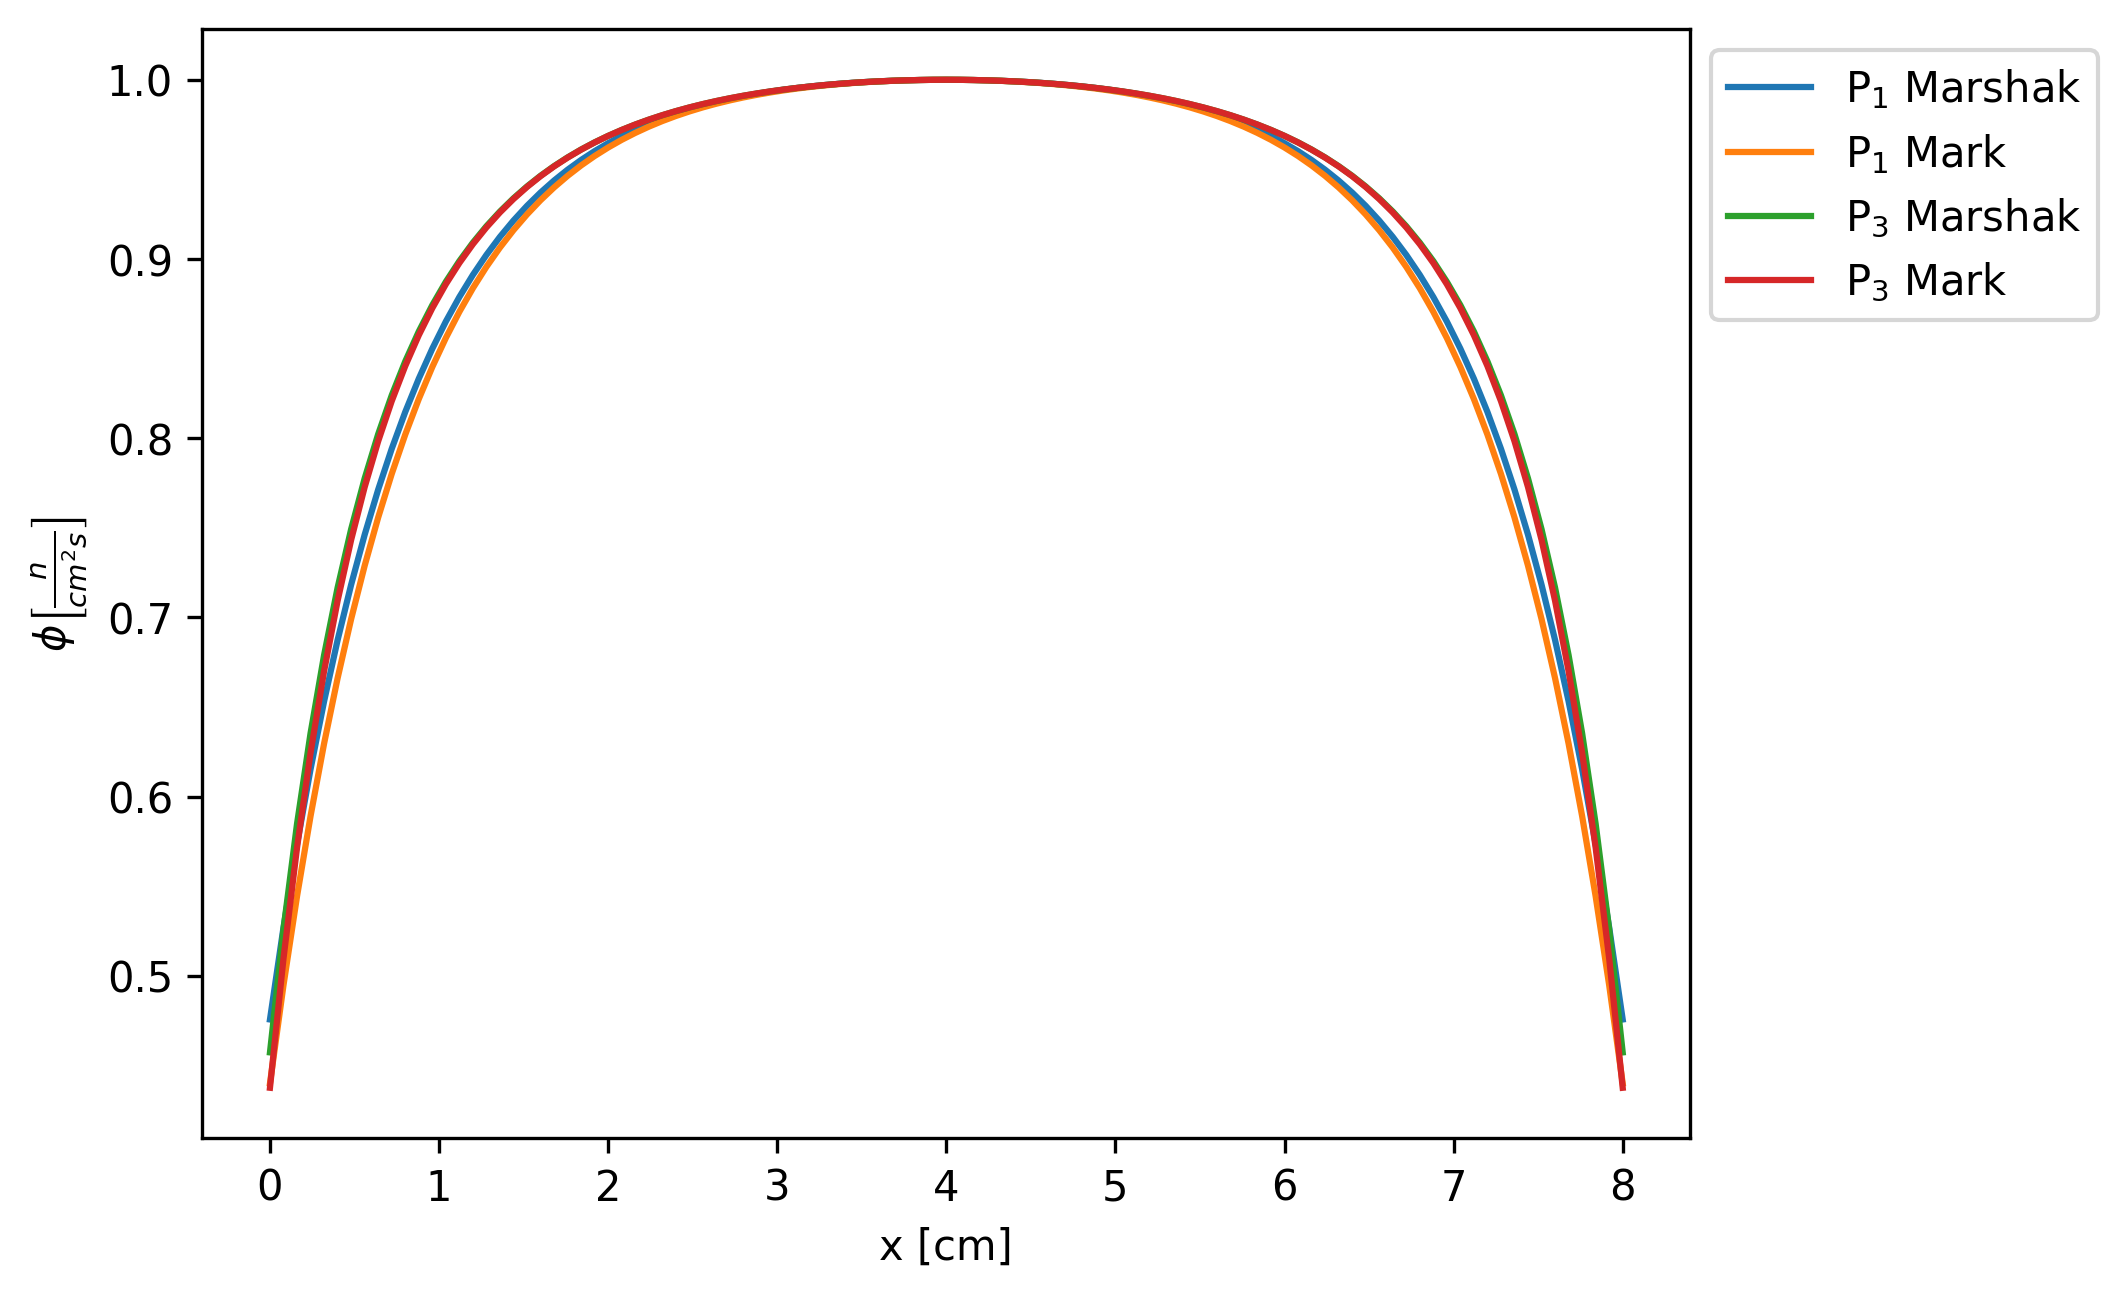
\includegraphics[width=8cm,height=8cm,keepaspectratio]{out.png}}       
        \subfigure[Reduced range plot. \label{fig:b}]{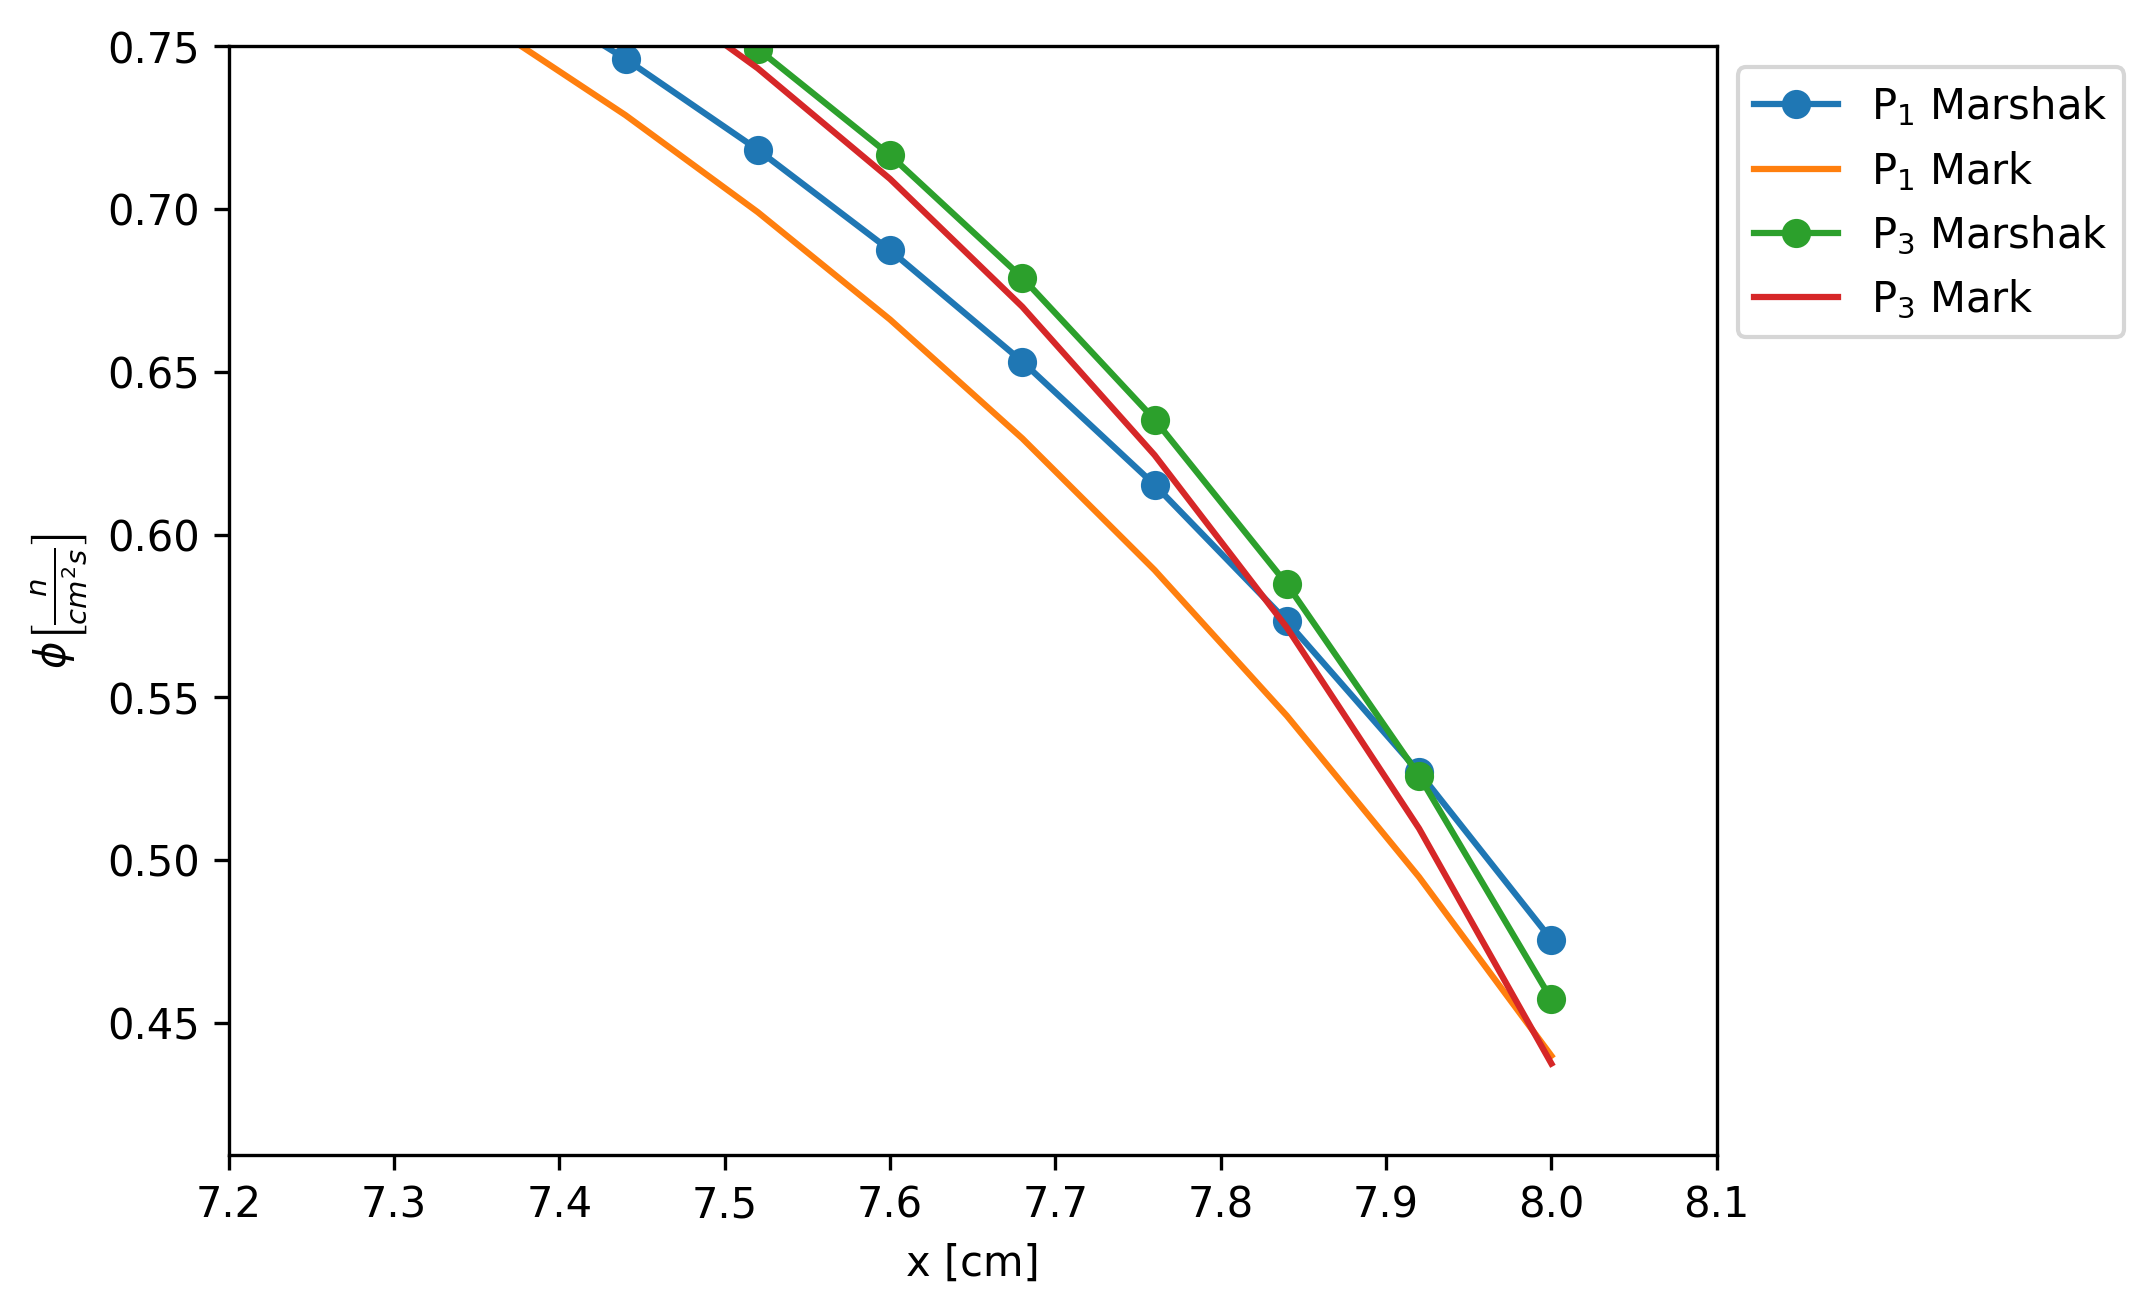
\includegraphics[width=8cm,height=8cm,keepaspectratio]{out-zoom.png}}
        \caption{Scalar flux normalized to maximum value.}
        \label{fig:results}
\end{figure}

\section{Conclusions}
In order to conduct the computer project, I had to understand the basics of the P$_N$ method.
The results help visualize some characteristics of the approximations.
Using a higher-order P$_N$ approximation better preserves the neutrons inside the domain.
Using a higher-order P$_N$ approximation also requires a more elaborate solver.
Choosing a Marshak boundary condition better conserves the neutrons inside the domain.
This type of boundary condition also requires a more elaborate formulation.

\clearpage
\bibliographystyle{plain}
% \bibliography{bibliography}
\end{document}

% \begin{figure}[h!]
%         \centering
%         \subfigure[Solved using FE.]{\includegraphics[width=8cm,height=8cm,keepaspectratio]{output6FE2b.png}}       
%         \subfigure[Solved using BE.]{\includegraphics[width=8cm,height=8cm,keepaspectratio]{output6BE2b.png}}
%         \caption{Power response for the sinusoidal reactivity in eq. \ref{sine2rho} for 6 Groups, $\Delta t = 1 ms$.}
%         \label{Output6-2b}
% \end{figure}

% \begin{figure}[h!]
%         \centering
%         \includegraphics[width=8cm,height=8cm,keepaspectratio]{AnalyticalSine1.png}
%         \caption{Analytical solution of $P(t)$ for the sinusoidal reactivity in eq. \ref{sine1rho}.}
%         \label{AnalyticSine}
% \end{figure}

% \begin{align}
%     0 &= D \nabla^2 \phi - \Sigma_a \phi + \nu \Sigma_f \phi \label{eq:diffusion} \\
%     D &\simeq \frac{1}{3 \Sigma_t}    \notag
%     \intertext{where}
%     D &= \mbox{Diffusion coefficient} \notag \\
%     \Sigma_t &= \mbox{Macroscopic total cross-section} \notag \\
%     \Sigma_a &= \mbox{Macroscopic absorption cross-section} \notag \\
%     \Sigma_f &= \mbox{Macroscopic fission cross-section} \notag \\
%     \nu  &= \mbox{Average number of neutrons born by fission.} \notag \\
% \end{align}

% \usepackage{booktabs}
% \begin{table}[htbp!]
%   \centering
%   \caption{.}
%   \begin{tabular}{lcc}
%   \toprule
%                  & Value & Units   \\
%   \midrule
%   Slab thickness & 8     & cm      \\
%   $\Sigma_t$     & 1.0   & 1/cm    \\
%   $\Sigma_{s0}$  & 0.4   & 1/cm    \\
%   $\Sigma_{s1}$  & 0.1   & 1/cm    \\
%   $\Sigma_{s2}$  & 0.1   & 1/cm    \\
%   $\Sigma_{s3}$  & 0.1   & 1/cm    \\
%   q$_0$          & 1     & n/cm$^{3}$/s \\

%   \bottomrule
%   \end{tabular}
%   \label{tab:parameters}
% \end{table}